\documentclass{article}
\usepackage[utf8]{inputenc}
\usepackage[english]{babel}
\usepackage{fancyhdr}
\usepackage{graphicx}
 
\pagestyle{plain}
\fancyhf{}
\rhead{Version: 1.4}
\chead{Date: 2018-10-17, Doc. Number: PUSS18002}
\lhead{Resp.: SG}
\title{SRS - Software Requirements Specification}
\usepackage{enumitem}
\usepackage{lipsum}
\begin{document}

\author{SG}

\maketitle
\thispagestyle{fancy}
\tableofcontents
\newpage

\section*{Document history}
 \begin{tabular}{||c c c c||} 
 \hline
 Version & Date & Resp & Description \\ [0.5ex] 
 \hline\hline
 0.1 & 2018-09-13 & SG & Draft version \\ 
 0.2 & 2018-09-14 & SG & Draft version 2 \\
 0.3 & 2018-09-27 & SG & Draft version 3 \\
 1.0 & 2018-10-02 & SG & Baseline \\
 1.1 & 2018-10-08 & SG & Requirement 6.3.3 expired \\
 1.2 & 2018-10-08 & SG & Requirement 6.6.3, 6.6.4 replaced \\
 1.3 & 2018-10-08 & SG & Requirement 6.4.5 replaced \\
 1.4 & 2018-10-17 & SG & Requirement 6.2.3, 6.2.5 expired, 6.1.3 replaced\\
 \hline
 

\end{tabular}

\section{Introduction}
This document describes the requirements for the the system. It is a system that helps commuters car pool between cities. The users should be able to add the routes they will be driving and search for routes they would like to ride with somebody.

The system is developed by group 5 of the course ETSN05 2018.

\section{Reference documents}
There are no referenced documents for this version.
\section{Background and goals}

\subsection{Main goals}
The main goal of the system is to make it easier for commuters to car pool. This would hopefully reduce traffic in heavily trafficked areas and make the the commuting less stressful for everyone.  
\subsection{Actors}
There are two main actors using the system

\textbf{User:} The users can be divided into two different roles, the driver and the commuter. Each physical person can have either role, although one person can never have both roles at the same time.

\textbf{Administrator:} The administrator is a special case user of the system. The administrator can add and remove users, rides and locations from the system. 

\section{Terminology}
\textbf{username:} The unique name of a user inside the system.
\\
\textbf{password:} A word or phrase used for authentication by the user.
\\
\textbf{ride:} Information about who is going to drive as well as from where to where, departure time, arrival time, and the number of seats available.

\section{Context and activity diagram}
The context diagram displayed in Figure \ref{fig:context} shows the interaction of the system's components and users on a high level.
\begin{figure}
  \centering
  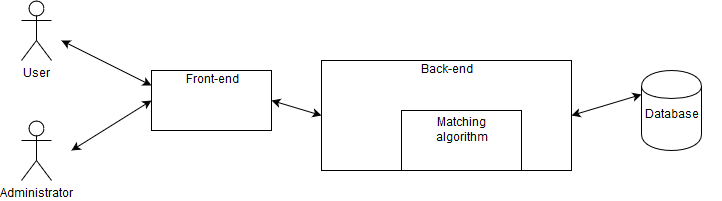
\includegraphics[scale=0.45]{Contextdiagram.png}
  \caption{Context diagram}
  \label{fig:context}
\end{figure}
\\ \\ 
Figure \ref{fig:activity} shows an activity diagram of the system.
\section{Functional requirements}

\begin{figure}
  \centering
  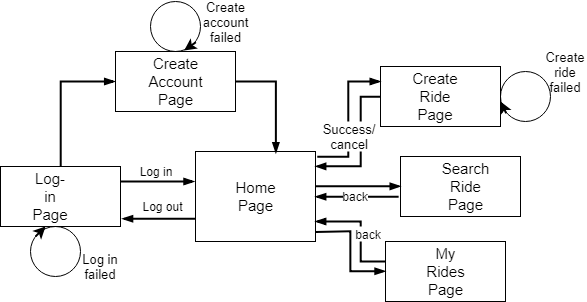
\includegraphics[scale=0.6]{forSRS.png}
  \caption{Activity diagram of the system.}
  \label{fig:activity}
\end{figure}

\subsection{Creating account}
\mbox{}\\
\textbf{Requirement 6.1.1} Scenario 6.1.1 should be supported by the system.
\\ \\
\textbf{Scenario 6.1.1} The user creates an account. Precondition: User is not logged in. 
\begin{enumerate}
    \item The program starts.
    \item The user presses the "new account"-button. 
    \item The user is taken to the "create account"-screen.
    \item The user is asked to provide the following:
        \begin{itemize}
            \item username,
            \item email,
            \item password.
        \end{itemize}
    \item The user provides username, email and password and presses create account.
    \item An account with the given information is saved to the database. The information is stored encrypted.
    \item The user is redirected to the "home"-screen.
\end{enumerate}
\mbox{}\\
\textbf{Requirement 6.1.2} Scenario 6.1.2 should be supported by the system.
\\ \\
\textbf{Scenario 6.1.2} The user tries to create an account with an illegal username, email or password (see 6.6)
\begin{enumerate}
    \item The program starts.
    \item The user presses the "new account"-button and is taken to the "create account"-screen.
   \item The user is asked to provide the following:
        \begin{itemize}
            \item username,
            \item email,
            \item password.
        \end{itemize}
    \item The user enters illegal information, or no information at all, to either of the following: 
        \begin{itemize}
            \item username,
            \item email,
            \item password.
        \end{itemize}
    \item An account is not created and a message is displayed stating "Invalid information given" as well as an "OK"-button. 
    \item The user presses the "OK"-button 
    \item The user is taken back to the "create account"-screen.
\end{enumerate}
\mbox{}\\
\textbf{Requirement 6.1.3} Expired, replaced by requirement 6.1.5.
\\ \\
\textbf{Requirement 6.1.4} Every account should have a unique email and username.
\\ \\
\textbf{Requirement 6.1.5} Scenario 6.1.5 should be supported by the system.
\\ \\
\textbf{Scenario 6.1.5} The user tries to create an account with an already occupied email or username.
\\ 
\begin{enumerate}
    \item The program starts.
    \item The user presses the "new account"-button and is taken to the "create account"-screen.
    \item The user is asked to provide the following: 
        \begin{itemize}
            \item username,
            \item email,
            \item password.
        \end{itemize}
    \item The user enters a username or an e-mail address already in use.
    \item An account is not created and a message is displayed stating "Email or username already in use" as well as an "OK"-button. 
    \item The user presses the "OK"-button.
    \item The user is taken back to the "create account"-screen
\end{enumerate}

\subsection{Log in and log out}
\textbf{Requirement 6.2.1} Scenario 6.2.1 should be supported by the system.
\\ \\
\textbf{Scenario 6.2.1} The user logs in. Precondition: User is not logged in. 
\begin{enumerate}
    \item The program starts
    \item The user is asked to provide username and password
    \item The user provides username and password and presses the "log in"-button.
    \item The user is directed to the "home"-screen.
\end{enumerate}
\mbox{}\
%\textbf{Scenario 6.2.2} The user fails to log in. Precondition: User is not logged in. 
%\begin{enumerate}
%    \item The program starts.
%    \item The user is asked to provide username and password
%    \item The user provides username and/or password incorrectly.
%    \item "Incorrect username or password" is displayed to the user.
%\end{enumerate}
\textbf{Requirement 6.2.2} Scenario 6.2.2 should be supported by the system.
\\ \\
\textbf{Scenario 6.2.2} The user tries to log in with an incorrect combination of username and password.
\begin{enumerate}
    \item The user enters an incorrect
    \begin{enumerate}[label=(\alph*)]
        \item username
        \item password
    \end{enumerate}
    \item an error message will be displayed, stating "Incorrect username or password"
\end{enumerate}
\mbox{}\\ \\
\textbf{Requirement 6.2.3} Expired
\\ \\
\textbf{Requirement 6.2.4} Scenario 6.2.4 should be supported by the system.
\\ \\
\textbf{Scenario 6.2.4} The user logs out. Precondition: The user is logged in.
\begin{enumerate}
    \item The user is presented with a "log out"-button.
    \item The user presses the "log out"-button.
    \item The user is taken back to the "log in"-screen.
\end{enumerate}
\mbox{}\\
\textbf{Requirement 6.2.5} Expired.
\subsection{Creating rides}
\textbf{Requirement 6.3.1} Scenario 6.3.1 should be supported by the system.
\\ \\
\textbf{Scenario 6.3.1} The user creates a ride. Precondition: The user is logged in. The user is not already booked in the specified time interval.
\\
\begin{enumerate}
    \item The user clicks the "Create ride"-button.
    \item The user is asked to provide the following:
        \begin{itemize}
            \item Departure time,
            \item arrival time, 
            \item number of seats available, 
            \item departure location,
            \item arrival location. 
        \end{itemize}
    \item The user provides the following:
        \begin{itemize}
            \item Departure time,
            \item arrival time, 
            \item number of seats available, 
            \item departure location,
            \item arrival location. 
        \end{itemize}
    \item The ride is saved and contains the departure time, arrival time, number of free seats, departure location,  arrival location and username of the ride creator.
    \item A message confirming that the ride was successfully created is displayed.
\end{enumerate}
\mbox{}\\ \\
\textbf{Requirement 6.3.2} Scenario 6.3.2 should be supported by the system.
\\ \\
\textbf{Scenario 6.3.2} The user provides illegal departure time, arrival time, number of free seats, departure location and/or arrival location. Precondition: The user is logged in and is creating a ride.

\begin{enumerate}
    \item The user clicks the "Create ride"-tab.
    \item The user is asked to provide the following:
        \begin{itemize}
            \item Departure time,
            \item arrival time, 
            \item number of seats available, 
            \item departure location,
            \item arrival location. 
        \end{itemize}
    \item The user provides illegal information (see definition of illegal information in \ref{section:data})  for one or more of the following arguments:
            \begin{itemize}
            \item Departure time,
            \item arrival time, 
            \item number of seats available, 
            \item departure location,
            \item arrival location. 
        \end{itemize}
    \item The ride is not created, and a message is displayed stating "The information entered was not correct".  
    \item The user is taken back to the "Create ride"-page.
    
\end{enumerate}
\mbox{}\\ \\
\textbf{Requirement 6.3.3} Expired. \\
\mbox{}\\ \\
\textbf{Requirement 6.3.4} Scenario 6.3.4 should be supported by the system.
\\ \\
\textbf{Scenario 6.3.4} The user tries to enter an invalid departure and/or arrival time.

\begin{enumerate}
    \item The user tries to enter a departure and/or arrival time which has already passed.
    \item The ride is not created and a message is displayed stating "Departure and/or arrival time has already passed".
    \item An "OK"-button is displayed, returning the user to the "create a new ride"-screen.
\end{enumerate}
\mbox{}\\ \\
\textbf{Requirement 6.3.5} Scenario 6.3.5 should be supported by the system.
\\ \\
\textbf{Scenario 6.3.5} The user tries to enter an invalid arrival time.

\begin{enumerate}
    \item The user tries to enter an arrival time that is before the departure time.
    \item The ride is not created, a message is displayed stating "arrival time needs to occur before the departure time" and an "OK"-button is displayed.
    \item The user clicks the "OK"-button and is taken back to "create a new ride"-screen.
\end{enumerate}
\mbox{}\\ \\
\textbf{Requirement 6.3.6} 
%The user should not be able to create a ride during  time where the user has indicated through other rides that the user will be traveling.
The user should not be able to create a ride that takes place at the same time as another ride that the user has signed up for.
\\ \\
%\textbf{Scenario 6.3.7} If the user tries to enter a departure time that is considered unreasonable based on previous rides(ex: the user has a arrival time in Helsingborg at 13.00 and tries to create a ride with a departure time at 13.05 from Stockholm) the ride is not created. A message is displayed stating "departure time considered unreasonable based on ride history" as well as an "ok"-button. The user presses the "ok"-button and is brought back to the create a ride screen. 
\\ \\
\subsection{Searching and joining rides}
\textbf{Requirement 6.4.1} Scenario 6.4.1 should be supported by the system.
\\ \\
\textbf{Scenario 6.4.1} The user searches for a ride and joins it. Precondition: The user is logged in.
\begin{enumerate}
    \item The user clicks the "search ride"-tab.
    \item The user is asked to provide departure time, departure location and arrival location. 
    \item The user provides provides departure time, departure location and arrival location.
    \item The user presses the "search"-button.
    \item The user is displayed a list of available rides. Each ride displays number of seats, number of free seats, username of all users who've signed up, roles of all users who've signed up, arrival time, departure time, arrival location and departure location.  
    \item The user presses the "join ride"-button attached to the ride.
    \item The ride is added to the users "My rides"-tab.
    \item A message stating that the ride was successfully joined is displayed.
\end{enumerate}
\textbf{Requirement 6.4.2} The user cannot join two rides that takes place during the same time.
\\ \\
\textbf{Requirement 6.4.3} When joining a ride, the user can see all of the usernames of the people added to the ride
\\ \\
\textbf{Requirement 6.4.4} The driver can kick other users from the ride. This removes the user from the ride and the ride from the kicked users "My rides"-tab.
\\ \\
\textbf{Requirement 6.4.5} Replaced by requirement 6.4.7
\\ \\
\textbf{Requirement 6.4.6} When searching for rides the rides are displayed according to the following rules:
\begin{enumerate}[label=(\alph*)]
    \item The system will only display rides which have a later departure time than the given departure time.
    \item The system will only show rides which contain a maximum 3 km difference between ride departure location and given departure location.
    \item The system will only show rides which contain a maximum 4 km difference between ride arrival location and given arrival location.
%\item The higher the ride rank, the higher up on the page it is displayed.
    \item Rides are partly ranked based on the following:
        \begin{itemize}
            \item the difference between given departure time and ride departure time,
            \item the distance between given arrival location and ride arrival time,
            \item number of seats available, 
            \item distance between given departure location and ride departure time.
        \end{itemize}
\end{enumerate}
\textbf{Requirement 6.4.7} The driver can ban users who have joined at least one of the drivers rides. The banned user will not be able to see this drivers rides in the future.
\\ \\


\subsection{Displaying joined rides and deleting a ride}
\textbf{Requirement 6.5.1} Scenario 6.5.1 should be supported by the system.
\\ \\
\textbf{Scenario 6.5.1} The driver deletes a ride. Precondition: The user is logged in and hosting a ride.
\begin{enumerate}
    \item The user clicks on the "My rides"-tab.
    \item The user is displayed a list of each ride the user has joined. Each ride displays the following:
            \begin{itemize}
            \item role of all users,
            \item username of all users who have joined the ride,
            \item total number of seats,
            \item number of free seats,
            \item arrival time,
            \item departure time,
            \item arrival location
            \item departure location.
        \end{itemize}       
    \item The user presses the "delete"-button attached to one of the rides created by the user.
    \item The ride is removed from the "My rides"-tab for all users who signed up to that ride. 
\end{enumerate} 
\mbox{}\\ \\
\textbf{Requirement 6.5.2} Scenario 6.5.2 should be supported by the system.
\\ \\
\textbf{Scenario 6.5.2} The user leaves a ride. Precondition: The user is logged in and has joined a ride.
\begin{enumerate}
    \item The user clicks on the "My rides"-tab.
    \item The user is displayed a list of each ride the user has joined. Each ride displays the following:
            \begin{itemize}
            \item role of all users,
            \item username of all users who have joined the ride,
            \item total number of seats,
            \item number of free seats,
            \item arrival time,
            \item departure time,
            \item arrival location
            \item departure location.
        \end{itemize} 
    \item The user presses the "leave"-button attached to one of the rides joined by the user.
    \item The ride is removed from the "My rides"-tab.
    \item The user is removed from the ride on the "My-ride"-tab of ther driver.
\end{enumerate} 
\mbox{}\\ \\


\subsection{Data} \label{section:data}
\textbf{Requirement 6.6.1} Usernames should consist of 3-20 characters, only numbers and English letters are allowed. 
\mbox{}\\
\\
\textbf{Requirement 6.6.2} Email should consist of 3-40 characters, only numbers, ascii-characters and traditional English letters are allowed. The email addresses must be of the format local-part@domain, e.g. "john.smith@example.com".
\mbox{}\\
\\
\textbf{Requirement 6.6.3} Replaced by requirement 6.6.8.
\\ \\
\textbf{Requirement 6.6.4} Replaced by requirement 6.6.9.
\\ \\
\textbf{Requirement 6.6.5} Arrival locations should only consist of letters, numbers and ascii-characters.
\\ \\
\textbf{Requirement 6.6.6} Departure locations should only consist of letters, numbers and ascii-characters.
\\ \\
\textbf{Requirement 6.6.7} Passwords should consist of 8-20 characters. Only numbers, special characters and English letters are allowed.
\\ \\
\textbf{Requirement 6.6.8} When creating a ride arrival time and departure should follow the format YYYY-MM-DD HH:MM, where YYYY,MM, DD, HH and MM are integers. YYYY represents the year, MM represents the month, DD represents the day, HH represents the hour and MM represents the minutes. 
\\ \\
\textbf{Requirement 6.6.9}  When searching for a ride arrival time and departure should follow the format YYYY-MM-DD HH:MM, where YYYY,MM, DD, HH and MM are integers. YYYY represents the year, MM represents the month, DD represents the day, HH represents the hour and MM represents the minutes. 

\subsection{Administration}
\textbf{Requirement 6.7.1} Admin users should be able to add users to the system.
\\ \\
\textbf{Requirement 6.7.2} Admin users should be able to ban users from using the application.
\\ \\
\textbf{Requirement 6.7.3} Admin users should be able to remove users from the system.
\\ \\
\textbf{Requirement 6.7.4} Admin users should be able to see all users, rides and locations.
\\ \\
\textbf{Requirement 6.7.5} Admin users should be able to delete existing commute rides.

\subsection{User roles}
\textbf{Requirement 6.8.1} A user cannot be a driver and passenger at the same time on any specific ride.

\section{Quality requirements}
\textbf{Requirement 7.1} At least 80\% of the code should be covered by unit-tests
\\ \\
\textbf{Requirement 7.2} Knowledge corresponding to the knowledge goals of EDAA45 / EDA011 / EDA016 / EDA017 / EDAA20, and a basic knowledge of SQL and JavaScript should be sufficient in order to understand, maintain, and further develop the system
\\ \\
%\textbf{Requirement 7.3.} 4 out of 5 students studying computer science at LTH should understand how to use the system within 10 seconds when sitting at a computer with the web-app opened.
\textbf{Requirement 7.3} 4 out of 5 student studying computer science at LTH should be able to create or join rides within 20 seconds when sitting at a computer with the web-app opened.
\\ \\
%Vet ej om det är möljigt? Kanske ska begränsa till 1-2 

\textbf{Requirement 7.5} When the system is used in one of the computer rooms in E-Huset, LTH, the response to any request should in at least 90\% of all cases be given within 2.0 seconds.
\\ \\
\textbf{Requirement 7.6} The system's capacity should be 1000 accounts.

\section{Project requirements}


\textbf{Requirement 8.1} The system's back-end should be developed in Java
\\ \\
\textbf{Requirement 8.2} The system's front-end should be developed in JavaScript
\\ \\
\textbf{Requirement 8.3} A SQL database should be used to store data.

\section{Delivery requirements}
\textbf{Requirement 9.1} The application should work with Google Chrome on computers running Windows 10, Ubuntu 18.04 or MacOS 10.13: "High Sierra".
\\ \\
\textbf{Requirement 9.2} The back end server should run on computers that run Ubuntu 18.04 and have Java 8 installed.
\\ \\ 
\textbf{Requirement 9.3} The database should be empty when the system is delivered.
\\ \\
\textbf{Requirement 9.4} A script that populates the database with test data should be included in the delivery.



\end{document}